\section{Falešné detekce}
\label{sec:Chapter63}

Na následujícím grafu \ref{fig:nets_false_detections} můžeme vidět falešné detekce mezi sítěmi na falešných snímcích z testovacího datasetu:

\begin{figure}[H]
\centering
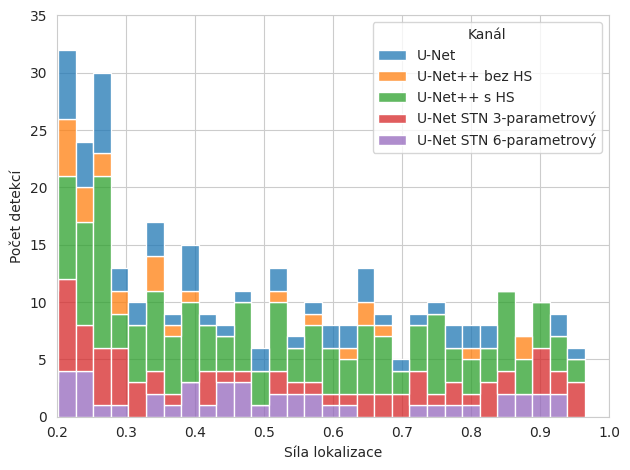
\includegraphics[width=0.8\textwidth,keepaspectratio]{Figures/plots/recall_graph_a.png}
\caption[Falešné detekce mezi sítěmi]{Falešné detekce mezi sítěmi}
\label{fig:nets_false_detections}
\end{figure}

V grafu \ref{fig:nets_false_detections} je k povšimnutí hned několik zajímavých trendů, blíže se na tyto data můžeme podívat v následující tabulce \ref{tab:false_detections}:

\begin{table}[H]
    \centering
    \begin{tabular}{llllllllll}
    \toprule
    & 0.2 & 0.3 & 0.4 & 0.5 & 0.6 & 0.7 & 0.8 & 0.9 \\
    \midrule
    U-Net & 59 & 39 & 30 & 24 & 18 & 12 & 5 & 3 \\
    U-Net++ bez HS & 27 & 15 & 10 & 9 & 7 & 3 & 3 & 0 \\
    U-Net++ s HS & 149 & 113 & 92 & 75 & 55 & 39 & 24 & 8 \\
    U-Net STN 3-parametrový & 67 & 44 & 38 & 33 & 29 & 23 & 15 & 9 \\
    U-Net STN 6-parametrový & 44 & 35 & 29 & 20 & 14 & 12 & 9 & 4 \\
    \bottomrule
    \end{tabular}
    \caption[Falešné detekce v závislosti na síle detekce]{Falešné detekce v závislosti na síle detekce mezi sítěmi}
    \label{tab:false_detections}
\end{table}

Na základě předvedených dat můžeme vidět, že síť \textbf{U-Net++ bez supervize} dosahuje nejlepších výsledků, kde dokonce nad hodnotu 0,9 nevidíme žádné falešné detekce. Model U-Net a U-Net STN s 6 parametry následují na druhém místě.  K povšimnutí je avšak zajímavé zhoršení  U-Net STN s 3 p. Také i verze s 6 p. na jistých milnících vykazuje horší výsledky oproti původní síti U-Net, avšak jen mírně.

Taky můžeme vidět, že počet falešných detekcí má lineární převahu v rozsahu [0,9...0,2] síly lokalizace, od hodnoty 0,2 nastává průlom.
\endinput
